%!TEX root = ../Testspezifikation.tex

\chapter{Testplan}

Im Folgenden wird der Testplan für \NewsGenie erläutert. Einzelne Komponenten
und ihre Funktionsweise, sowie die daraus resultierende Teststrategie werden
vorgestellt. 

\NewsGenie setzt mit Sprachsteuerung auf ein Eingabemedium, für das dem Benutzer
keine eigenen Strategien zur Fehlerbehandlung zur Verfügung stehen (am
Bildschirm zum Beispiel das Schließen und erneute Öffnen des Programms),
deshalb muss besonderes Augenmerk auf die Stabilität, Fehlertoleranz und einfache
Bedienbarkeit dieser Schnittstelle gelegt werden.

\section{Zu testende Komponenten}

\NewsGenie wird aus einem Client und verschiedenen Serverkomponenten bestehen.
Wie in Abb. \ref{komponenten} dargestellt handelt es sich dabei um

\begin{description}
\item[Client] Läuft auf einem Raspberry Pi Einplatinencomputer und
wird die direkte Interaktion mit dem Benutzer übernehmen, sowie dessen Anfragen
an den Server weiterleiten
\item[Crawler] Eine Serveranwendung, die im Hintergrund die vom Benutzer
hinzugefügten RSS-Feeds durchsucht und indexiert. Bereitet die Daten für den
QueryProcessor auf.
\item[QueryProcessor] Nimmt die Anfragen der Clients entgegen und generiert
möglichst präzise Antworten auf die gestellten Fragen. Dabei greift er auf die
vom Crawler indexierten Daten zu.
\item[Webinterface] Ist für die Registrierung und die Einstellungen der Nutzer
zuständig. Außerdem bietet das Webinterface Funktionen zur textbasierten Anfrage
des QueryProcessors.
\item[Datenbank] Verbindet die einzelnen Komponenten und muss deshalb ein
robustes Schema bieten, auf das alle Anwendungen gleichzeitig zugreifen können.
\end{description}

\begin{figure}[h]
\centering
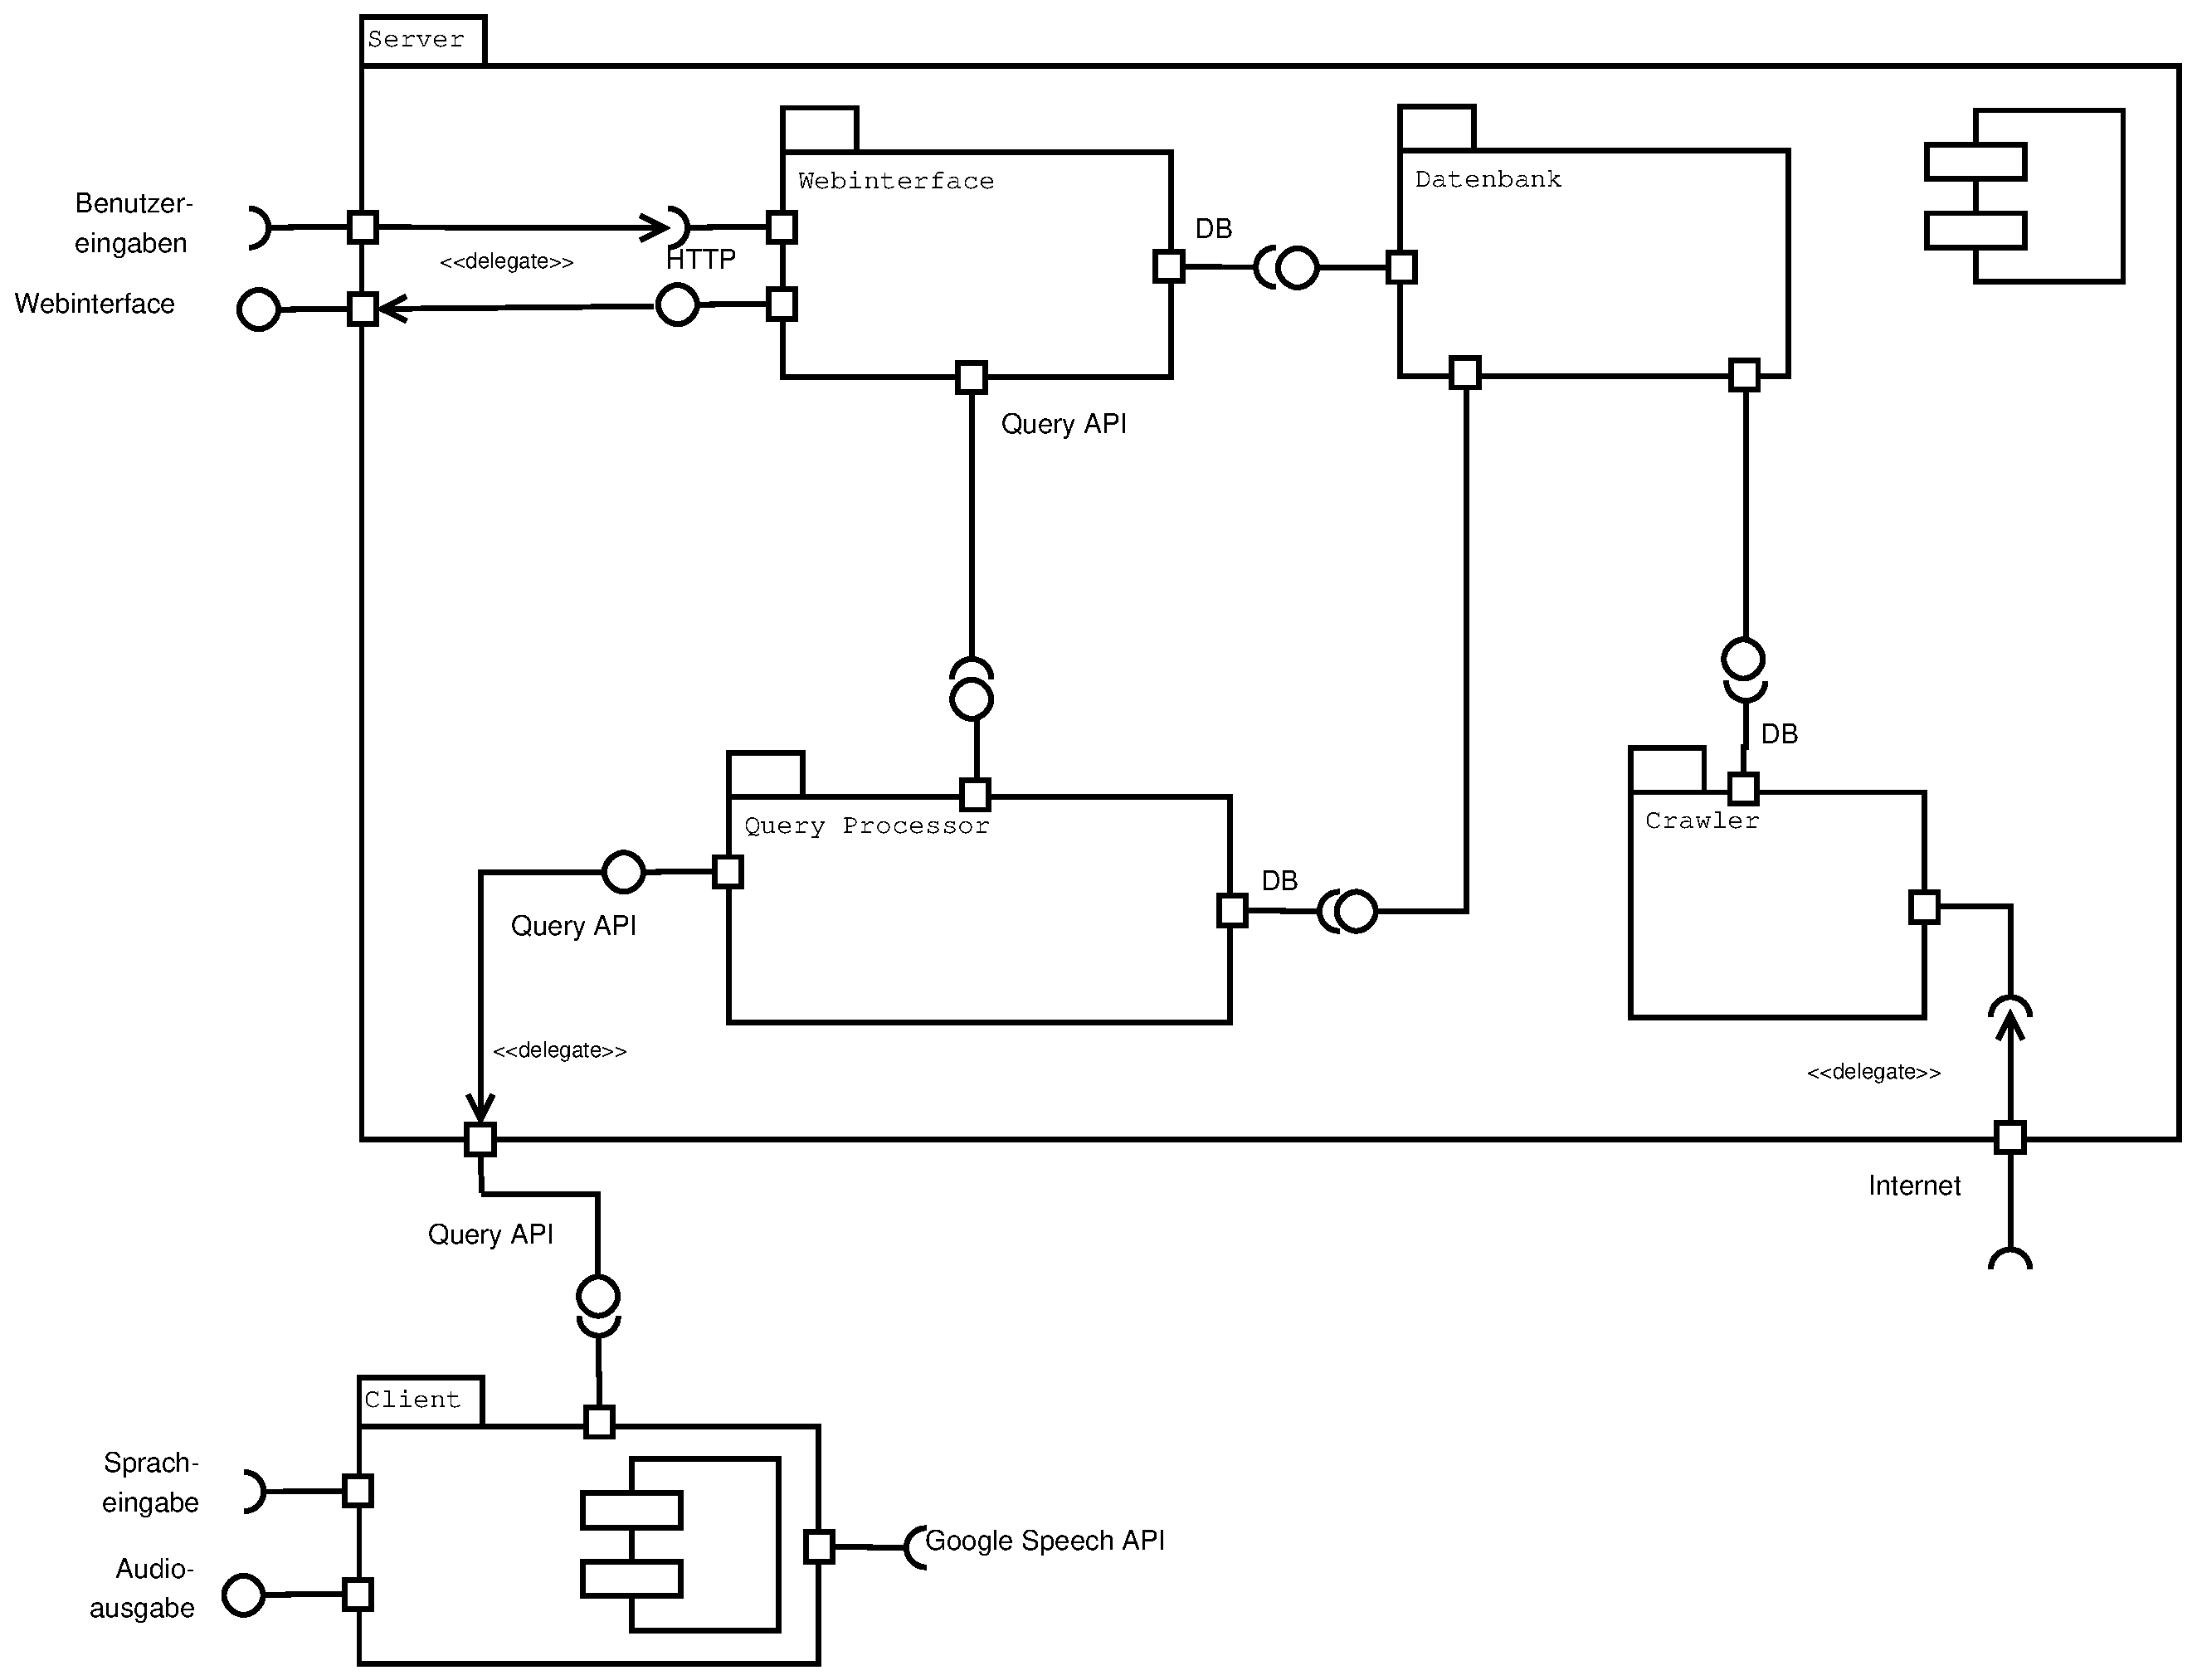
\includegraphics[width=1\textwidth]{Testspezifikation/testplan/komponenten}
\caption{Komponentendiagramm, \textit{Architektur von \NewsGenie}
\label{komponenten}}
\end{figure}

\pagebreak
\section{Zu testende Funktionen/Merkmale}

\begin{itemize}
\item \ref{RM1} Ein- und Ausgabe in natürlicher Sprache:  Das System ist in der Lage verbal mit dem Benutzer zu kommunizieren.
Um dies zu ermöglichen, kann es gesprochene Anfragen aufnehmen und verarbeiten sowie Antworten formulieren und leicht verständlich ausgeben.
\item \ref{RM2} Interaktives Verhalten: Das System grenzt Anfragen mit Ja-/Nein-Fragen ein, bricht die Sprachausgabe bei einem Stopp-Befehl ab und erlaubt negatives Feedback.
\item \ref{RM4} Benutzerschnittstelle: Das Webinterface bietet die Möglichkeit, Textanfragen zu stellen und die Resultate manuell zu validieren.
\item \ref{RM5} Backend: Nachrichtendaten werden in einem \glqq Triplestore\grqq\ mit \glqq Inverted Indexes\grqq\ gespeichert um effiziente Volltextsuche zu ermöglichen. Zu einer Anfrage werden ausschließlich dazu passende Artikel ausgegeben.
\item \ref{F10} Ausgabe von natürlicher Sprache: Der Client kann natürliche Sprache ausgeben.
\item \ref{F11} Aufnahme von natürlicher Sprache: Der Client kann natürliche Sprache aufnehmen.
\item \ref{F12} Umwandlung von Sprache in Text: Das System kann Sprachdateien in Text umwandeln.
\item \ref{F13} Umwandlung von Text in Sprache: Das System kann Text in Sprachdateien umwandeln.
\item \ref{F30}, \ref{F20} Anfrage stellen: Wenn der Benutzer am Client eingeloggt ist, kann er Anfragen stellen und erhält eine sinnvolle Antwort.
\item \ref{F30} Client Login: Ein Benutzer kann sich am Client einloggen.
\item \ref{F30}, \ref{F31} Client Logout: Nach einem Login am Client kann sich ein Benutzer wieder ausloggen.
\item \ref{F40} News-Crawling: Neue Artikel werden regelmäßig in das System aufgenommen.
\item \ref{F50} Registrierung: Neue Benutzer können sich registrieren.
\item \ref{F60} Webinterface Login: Benutzer können sich am Webinterface einloggen.
\item \ref{F60}, \ref{F61} Webinterface Logout: Nach einem Login am Webinterface kann sich ein Benutzer wieder ausloggen.
\item \ref{F60}, \ref{F70} Feed-Liste anzeigen: Eingeloggten Benutzern wird eine Liste ihrer abonnierten Feeds angezeigt.
\item \ref{F60}, \ref{F71} Feed hinzufügen: Eingeloggte Benutzer können neue Feeds abonnieren.
\item \ref{F60}, \ref{F71}, \ref{F72} Feed entfernen: Eingeloggte Benutzer können zuvor abonnierte Feeds wieder entfernen.
\item \ref{F60}, \ref{F80} Passwort ändern: Eingeloggte Benutzer können ihr Passwort ändern.
\item \ref{F81} Passwort Wiederherstellung: Benutzer können ihr Passwort wiederherstellen.
\item \ref{F60}, \ref{F90} Rolle wechseln: Eingeloggte Administratoren können die Rolle eines anderen Benutzers annehmen.
\item \ref{F60}, \ref{F100} Benutzer-Liste anzeigen: Eingeloggten Administratoren wird eine Liste aller Benutzer angezeigt.
\item \ref{F60}, \ref{F110} Benutzer löschen: Eingeloggte Benutzer haben die Möglichkeit, ihren Account zu löschen.
\item \ref{F60}, \ref{F120} Eingeloggte Benutzer können Textanfragen stellen und die Resultate manuell validieren.
\item \ref{Q10} Maximale Antwortzeit: Auf jede Benutzereingabe erfolgt innerhalb von maximal fünf Sekunden eine Antwort.
\item \ref{Q20} Anwenderfreundlichkeit: Das Produkt ist für Benutzer ohne EDV-Vorkenntnisse intuitiv bedienbar.
\item \ref{Q30} Robustheit: Fehlerhafte Eingaben bringen das Produkt nicht zum Absturz.
\item \ref{Q40} Relevanz: Benutzer erhalten nur für sie relevante Nachrichten.
\item \ref{Q50} Ressourcenverbrauch: Der Client funktioniert ohne Einschränkungen auf einem Raspberry Pi.
\end{itemize}
 

\section{Nicht zu testende Funktionen}

Die Anforderung \ref{RM3} \glqq Das System muss die englische Sprache unterstützen\grqq\ wird von uns nicht separat getestet, da sie sich auf alle Funktionen bezieht. Die Erfüllung der Anforderung wird dadurch beim Test der einzelnen Funktionen überprüft.\\
Außerdem setzen wir hinreichende Tests bei allen von Drittanbietern entwickelten Bibliotheken und Systemen voraus und testen diese nicht selbst.\\
Insbesondere sind dies:

\begin{itemize}
\item Apache openNLP
\item Apache Lucene
\item akka
\item playFramework
\item OpenLink Virtuoso
\item Google-Speech-API
\item Raspbian
\item Debian
\end{itemize}

\section{Vorgehen}

Die Software des \NewsGenies kann in vier Bereiche getrennt und im einzelnen
getestet werden:
Funktionalitäten des Clients, Funktionalitäten des Servers, Funktionalitäten des
Webinterfaces und schließlich das Zusammenspiel des Client-Server-Systems. In
folgenden Schritten wird beim Testen vorgegangen:

\begin{enumerate}

\item{Komponententest}\\
Alle Komponenten von \NewsGenie können mit JUnit-Tests überprüft werden.
Während der Implementierung werden bereits Blackbox-Testfälle vom jeweiligen Autor
erstellt und im Test-First-Verfahren begleitend zur Implementierung
durchgeführt. Nach Abschluss der Implementierung einer Klasse ist so bereits ihre (unabhängige) Funktionalität sichergestellt.
\item{Integrationstest}\\
Wurde eine Komponente fertiggestellt und erfolgreich getestet, folgt nach
dem Bottom-Up-Prinzip die Integration in \NewsGenie. Dabei wird durch das
Ausführen von \NewsGenie der Integrationstest sowie die Funktionaliät geprüft.
In welcher Reihenfolge die Komponenten unter Berücksichtigung ihrer Abhängigkeit integriert
werden, wird zu einem späteren Zeitpunkt konkretisiert.
\item{Systemtest}\\
Die Anforderungen des Systems aus dem Pflichtenheft werden geprüft, indem sie
auf dem System mindestens einmal korrekt ausgeführt werden. Dabei wird ein Client
und ein gestartetes Webinterface benötigt. Probleme oder Auffälligkeiten werden
dokumentiert und gegebenenfalls behoben.
\item{Abnahmetest}\\
Die Anforderung \ref{RM5} \glqq Backend\grqq\ und die damit verbundene Funktion \ref{F40} \glqq News-Crawling\grqq\ können nicht vom Kunden direkt getestet werden. Um die Korrektheit der Implementierung zu zeigen, legen wir eine Log-Datei vor, die zeigt, wann welche Artikel in die Datenbank aufgenommen wurden. \\
Alle anderen Funktionen kann der Kunde selbst vor Ort testen. Dazu wird er sich zunächst einen Account anlegen, sich mit diesem einloggen und alle Funktionen des Webinterfaces sowie des Clients nacheinander ausprobieren. Bei diesem Vorgang erhält der Kunde auch einen guten Eindruck der Qualitätsmerkmale \ref{Q10} \glqq Maximale Antwortzeit\grqq\, \ref{Q20} \glqq Anwenderfreundlichkeit\grqq\, \ref{Q40} \glqq Relevanz\grqq\ und \ref{Q50} \glqq Ressourcenverbrauch\grqq . Zum Testen von Qualitätsmerkmal \ref{Q30} \glqq Robustheit\grqq\ ist eine größere Anzahl an Probedurchläufen nötig, die wir in Form einer Umfrage gestalten werden. Bei dieser werden sowohl \ref{Q20} \glqq Anwenderfreundlichkeit\grqq\ als auch \ref{Q30} \glqq Robustheit\grqq\ getestet.
\end{enumerate}


\section{Testumgebung}

Sowie für die Entwicklung als auch den Abnahmetest und die weitere Verwendung wird die Serversoftware auf einem Server des IfIs ausgeführt und ein Raspberry Pi als Client verwendet. Zum Testen muss auf beiden Systemen eine JUnit-Testsuite installiert sein.
